\documentclass[11pt]{article}
\usepackage[utf8]{inputenc} % Para caracteres en espa�ol
\usepackage{amsmath,amsthm,amsfonts,amssymb,amscd}
\usepackage{multirow,booktabs}
\usepackage[table]{xcolor}
\usepackage{fullpage}
\usepackage{lastpage}
\usepackage{enumitem}
\usepackage{multicol}
\usepackage{fancyhdr}
\usepackage{mathrsfs}
\usepackage{wrapfig}
\usepackage{setspace}
\usepackage{esvect}
\usepackage{calc}
\usepackage{multicol}
\usepackage{cancel}
\usepackage{graphicx}
\graphicspath{ {pictures/} }
\usepackage[retainorgcmds]{IEEEtrantools}
\usepackage[margin=3cm]{geometry}
\usepackage{amsmath}
\newlength{\tabcont}
\setlength{\parindent}{0.0in}
\setlength{\parskip}{0.05in}
\usepackage{empheq}
\usepackage{framed}
\usepackage[most]{tcolorbox}
\usepackage{xcolor}
\colorlet{shadecolor}{orange!15}
\parindent 0in
\parskip 12pt
\geometry{margin=1in, headsep=0.25in}
\theoremstyle{definition}
\newtheorem{defn}{Definition}
\newtheorem{reg}{Rule}
\newtheorem{exer}{Exercise}
\newtheorem{note}{Note}
\begin{document}
\setcounter{section}{0}
 \pagestyle{fancy}
\fancyhf{}
\rhead{AE370: Application Problems}
\begin{center}
\vspace{10mm}
\end{center}
{\LARGE \bf Application Problem 1:}\\ \\ \\
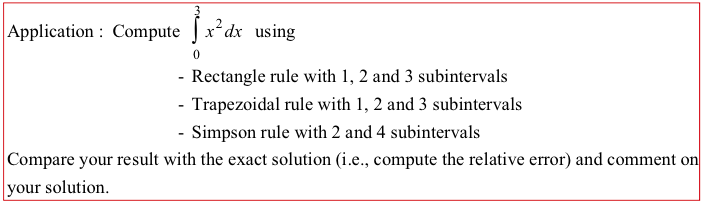
\includegraphics[scale=0.75]{1.png}
\begin{itemize}
\item \textbf{Exact Solution}
\\ \\ \\
\begin{equation*}
\begin{aligned}
y = \int_{0}^{3} x^2 \mathrm{d}x = \bigg[ \frac{1}{3} x^{3}\bigg]_{0}^{3} = 9
\end{aligned}
\end{equation*}
\begin{center}
\vspace{100mm}
\end{center}
\newpage
\item \textbf{Rectangle Rule Solution}
\newline
\begin{shaded}
\textbf{Rectangle Rule for Integration} \newline
\begin{equation*}
\int_{x_{i-1}}^{x_i} f(x) \mathrm{d}x \approx \sum_{i=1}^{n} \, h_{i} \, f(\frac{x_{i-1}+x_{i}}{2})
\end{equation*}
Where:
\begin{equation*}
\begin{split}
n &= \text{Number of Subintervals} \\
h_i & = (x_i - x_{i-1}) \\
h &= \frac{x_{\text{final}} - x_{\text{initial}}}{n} \\
& = \text{Length of a Single Subinterval} \\
\end{split}
\end{equation*}
\end{shaded}

\begin{equation*}
\begin{aligned}
\text{1 Subinterval:} &&&\\
& h = \frac{3-0}{1} = 3  &\text{therefore}& \qquad y = 3 \bigg(\frac{0+3}{2}\bigg)^2 = 6.75 \\
\text{2 Subintervals:} & \\
& h = \frac{3-0}{2} = 1.5 &\text{therefore}& \qquad y = 1.5 \bigg(\frac{0+1.5}{2}\bigg)^2 + 1.5 \bigg(\frac{1.5+3}{2}\bigg)^2 = 8.4375 \\
\text{3 Subintervals:} &\\
& h = \frac{3-0}{3} = 1 &\text{therefore}& \qquad  y = 1 \bigg(\frac{0+1}{2}\bigg)^2 + 1\bigg(\frac{1+2}{2}\bigg)^2 + 1\bigg(\frac{2+3}{2}\bigg)^2= 8.75 \\
\end{aligned}
\end{equation*}
\newpage
\item \textbf{Trapezoidal Rule  Solution}
\begin{shaded}
\textbf{Trapezoidal Rule for Integration} \newline
\begin{equation*}
\int_{x_{i-1}}^{x_i} f(x) \mathrm{d}x \approx \sum_{i=1}^{n} \, \frac{h_{i}}{2} \, \bigg(f(x_{i-1})+f(x_{i})\bigg)
\end{equation*}
Where:
\begin{equation*}
\begin{split}
n &= \text{Number of Intervals} \\
h_i & = (x_i - x_{i-1}) \\
h &= \frac{x_{\text{final}} - x_{\text{initial}}}{n} \\
& = \text{Length of a Single Subinterval}
\end{split}
\end{equation*}
\end{shaded}
\begin{equation*}
\begin{aligned}
\text{1 Subinterval:} &&&\\
& h = \frac{3-0}{1} = 3  &\text{therefore}& \qquad y = \frac{3}{2}\big(0^2+3^2\big) = 13.5 \\
\text{2 Subintervals:} & \\
& h = \frac{3-0}{2} = 1.5 &\text{therefore}& \qquad y = \frac{1.5}{2}\big(0^2+1.5^2\big)+\frac{1.5}{2}\big(1.5^2+3^2\big) = 10.125 \\
\text{3 Subintervals:} &\\
& h = \frac{3-0}{3} = 1 &\text{therefore}& \qquad  y = \frac{1}{2}\big(0^2+1^2\big)+frac{1}{2}\big(1^2+2^2\big)+frac{1}{2}\big(2^2+3^2\big) = 9.5 \\
\end{aligned}
\end{equation*}
\newpage
\item \textbf{Simpson Rule Solution}
\begin{shaded}
\textbf{Simpson Rule for Integration} \newline
\begin{equation*}
\int_{x_{i-1}}^{x_i} f(x) \mathrm{d}x \approx \frac{2}{3} \, I_{\text{rectangular}} + \frac{1}{3} \, I_{\text{trapezoidal}}
\end{equation*}
Where:
\begin{equation*}
\begin{split}
I_{\text{rectangular}} &= \text{Rectangle Rule Estimate} \\
I_{\text{trapezoidal}} &= \text{Trapezoidal Rule Estimate} \\
\end{split}
\end{equation*}
\end{shaded}
\begin{equation*}
\begin{aligned}
\text{2 Subintervals:} & \\
& h = \frac{3-0}{2} = 1.5 \\ \\
\text{therefore} & \\ \\
& \qquad I_{\text{rectangular}} = 1.5 \bigg(\frac{0+1.5}{2}\bigg)^2 + 1.5 \bigg(\frac{1.5+3}{2}\bigg)^2 = 8.4375 \\ \\
& \qquad I_{\text{trapezoidal}} = \frac{3-0}{2} = 1.5 = \frac{1.5}{2}\big(0^2+1.5^2\big)+\frac{1.5}{2}\big(1.5^2+3^2\big) = 10.125 \\ \\
\text{As a result}& \\ \\
&\qquad y = \frac{2}{3} \, I_{\text{rectangular}} + \frac{1}{3} \, I_{\text{trapezoidal}}\\ \\
&\qquad \, \, = \frac{2}{3} \, (8.4375) + \frac{1}{3} \, (10.125) \\ \\
&\qquad \, \,= 9 \qquad \leftarrow \text{This is our exact solution!}
\end{aligned}
\end{equation*}
\end{itemize}
\newpage
\section{Problem 2}
\newpage
%%%%%%%%%%%%%%%%%%%%%%%%%%%%%%%%%%%%%%%%%%%%%%%%%%%%%%%%
%%%%%%%%%%%%%%                         BASIC TEMPLATES                                %%%%%%%%%%%%%%
%%%%%%%%%%%%%%%%%%%%%%%%%%%%%%%%%%%%%%%%%%%%%%%%%%%%%%%%
\section{Basic Templates}
% Basic Note Guides
\begin{note} \textbf{This is how you make numbered notes}\end{note}
\begin{exer} \textbf{This is how you make numbered exercises}\end{exer}
\begin{defn} \textbf{This is how you make numbered definitions}\end{defn}
\begin{reg} \textbf{This is how you make numbered rules}\end{reg}

%Shaded Equations + Explainer
\begin{shaded}
\textbf{Simpson Rule for Integration} \newline
\begin{equation*}
\int_{x_{i-1}}^{x_i} f(x) \mathrm{d}x \approx \frac{2}{3} \, I_{\text{rectangular}} + \frac{1}{3} \, I_{\text{trapezoidal}}
\end{equation*}
Where:
\begin{equation*}
\begin{split}
I_{\text{Rectangular}} &= \text{Rectangle Rule Estimate} \\
I_{\text{Trapezoidal}} &= \text{Trapezoidal Rule Estimate} \\
\end{split}
\end{equation*}
\end{shaded}

%Insert Photo
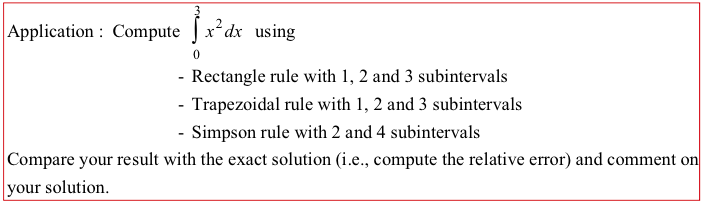
\includegraphics[scale=0.75]{1.png}

\end{document}